%% Los cap'itulos inician con \chapter{T'itulo}, estos aparecen numerados y
%% se incluyen en el 'indice general.
%%
%% Recuerda que aqu'i ya puedes escribir acentos como: 'a, 'e, 'i, etc.
%% La letra n con tilde es: 'n.

\chapter{Métodos}
%\setcounter{section}{1}
\section{Métodos estadísticos}

\subsection{Modelo AMMI}

\textbf{Modelo AMMI clásico}

El modelo AMMI es un modelo multiplicativo en el cual se expresa la respuesta de un genotipo en un ambiente de la siguiente forma:
\begin{center}
$y_{ij}= \mu +G_i + A_j + \sum_{k=1}^q \lambda_k \alpha_{ik} \gamma_{jk}$ \vspace{1cm} $ i=1,...,g$; $ j=1,...,a$ $q=min(g-1,a-1)$
\end{center}
donde 
\begin{itemize}
\item $y_{ij}$ es el caracter fenotípico evaluado (rendimiento o cualquier otro caracter de interes) del $i$-ésimo genotipo en el $j$-ésimo ambiente,
\item $\mu$ es la media general,
\item  $G_i$ es el efecto del $i$-ésimo genotipo,
\item $A_j$ es el efecto del $j$-ésimo ambiente
\item $\sum_{k=1}^q \lambda_k \alpha_{ik} \gamma_{jk}$ es la sumatoria de componentes multiplicativas utilizadas para modelar la IGA. Siendo, $\lambda_k$ el valor singular para la  $k$-ésima IPC $\alpha_{ik}$ y $\gamma_{jk}$ son los scores de las PC para el $i$-ésimo genotipo y el $j$-ésima ambiente para la $k$-ésima componente, respectivamente;
\end{itemize}

Los parámetros de IGA en el modelo AMMI se estiman por medio de la DVS de la matriz que contiene los residuos del modelo aditivo luego de ajustar por mínimos cuadrados el modelo de efectos principales.

Generalmente los dos primeros términos multiplicativos son suficientes para explicar los patrones de interacción; la variabilidad remanente se interpreta como ruido. 

Los patrones de interacción se pueden visualizar mediante los biplots \emph{Genotipe-Environment}, a menudo llamados biplots GE. El concepto del biplot fue presentado por Gabriel (1971), que consiste en una representación de las filas (individuos) y las columnas (variables) de una matriz de datos en un mismo gráfico. 

\textbf{Biplot GE}

En los modelos AMMI, el biplot GE ayuda a interpretar la variación producida por los efectos de la IGA. Se grafican en un sistema de coordenadas cartesianas de dos dimensiones los scores de los genotipos ($\alpha_{ik}$) y los ambientes ($\gamma_{jk}$), ponderados por la raíz cuadrada del autovalor correspondiente ($\lambda_k$).

Dado que los genotipos y los ambientes son definidos como vectores desde el origen (0,0) hasta sus scores, el biplot se interpreta en términos de las direcciones de vectores y sus proyecciones.\\

El módulo del vector de un ambiente da una idea de la contribución del mismo a la interacción. Los puntos de los genotipos que se encuentran próximos al origen indican que los mismos contribuyen poco a la interacción, es decir, se adaptan de igual manera a todos los ambientes. Puntos cercanos entre sí tienen patrones de interacción similares, mientras que puntos alejados entre sí tienen patrones diferentes. Cuando los marcadores (o puntos) de los ambientes y genotipos están próximos, es decir forman un aungulo $< 90^o$ ó $> 270^o$, indica que contribuyen positivamente a la interacción(hay una asociación positiva entre ese genotipo y ese ambiente); y mientras más alejados del origen se encuentre los marcadores, más fuerte será esa asociación. Una fuerte asociación positiva entre un genotipo y un ambiente se interpreta como que ese ambiente es muy favorable para ese genotipo. De manera similar, cuando los marcadores del genotipo y el ambiente están opuestos entre sí (forman un ángulo entre $90^o$ y $270^o$) se interpreta que ese ambiente es muy desfavorable para ese genotipo.\\


En la Figura \ref{fig:fig311}, se presenta un ejemplo de un biplot GE con 6 ambientes (A, B, C, D, E y F) y 10 genotipos (1, 2, 3, 4, 5, 6, 7, 8, 9 y 10). Se observa que la magnitud de los vectores de los ambientes A y E es mayor a la de los demás ambientes, es decir que esos dos ambientes son los que más contribuyen a la interacción. La cercanía de los marcadores de los genotipos 1 y 2 indica que esos genotipos tienen patrones de interacción similares, y a la vez, muy distintos a los del genotipo 4. Del biplot también se destacan las cercanías entre el genotipo 9 y el ambiente A, entre el genotipo 5 con el ambiente C, entre los genotipos 1 y 2 con el ambiente E, entre los genotipos 6, 7 y 10 con el ambiente F y entre el genotipo 4 con el ambiente D, lo que indica, debido a la gran distancia al origen, una fuerte asociación positiva entre esos genotipos y esos ambientes, es decir, esos ambientes son muy favorables para esos genotipos.\\

\begin{figure}[h]
	\begin{center}
		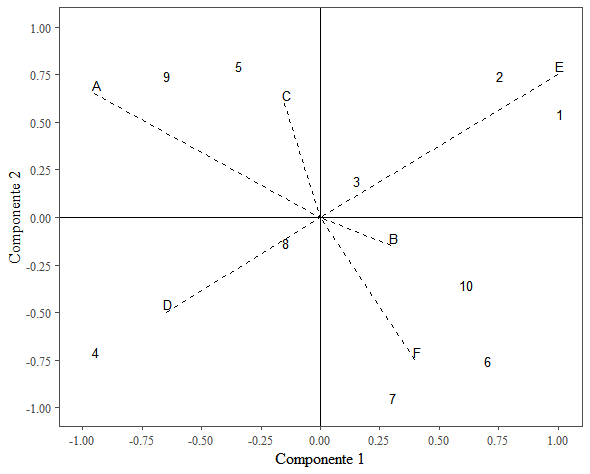
\includegraphics[width=10cm]{./Graficos/GE_biplot.png}
	\end{center}
	\caption{Ejemplo de un biplot GE}
	\label{fig:fig311}
\end{figure}

Entre las altas asociaciones negativas se puede mencionar a la del ambiente A con el genotipo 10 (marcadores opuestos en el biplot) y se interpreta que ese ambiente es considerablemente desfavorable para ese genotipo.\\

También se observa que los genotipos 3 y 8 están próximos al origen, lo que quiere decir que se adaptan en igual medida a todos los ambientes.


\textbf{Modelo AMMI robusto}

El modelo AMMI, en su forma estándar, asume que no hay valores atípicos en el conjunto de datos. La presencia de observaciones atípicas es más una regla que una excepción cuando se consideran datos agronómicos debido a errores de medición, algunas plagas / enfermedad que puede influir en algunos genotipos en un ambiente dado que resultando por ejemplo en un rendimiento inferior al esperado, o incluso debido a alguna característica inherente de los genotipos que se miden.

Rodrigues 2015 proponen una generalización robusta del modelo AMMI. La metología propuesta se puede obtener en dos etapas de la siguiente manera: primero ajustar la regresión robusta basada
en el estimador M-Huber \citep{Huber1981} para reemplazar el ANOVA; y luego utilizar un procedimiento SVD / PCA robusto para reemplazar el SVD estándar. En la segunda etapa, consideraron varios métodos dando lugar a total de cinco robustos: R-AMMI, H-AMMI, G-AMMI, L-AMMI, PP-AMMI. 

El empleo de la versión robusta del modelo AMMI puede ser extremadamente útil debido a que una mala representación de genotipos y ambientes en los biplots puede dar como resultado un mala decisión con respecto a qué genotipos seleccionar para un conjunto dado de ambientes (es decir, megaambientes; \cite{Gauch1997}; \cite{Yanetal2000}). A su vez, la elección de los genotipos incorrectos pueden provocar grandes pérdidas en términos de producción de rendimiento.

Debe tenerse en cuenta que los biplots robustos mantienen las características e interpretación estándar del modelo AMMI clásico.

\subsection{Modelo SREG}

El modelo SREG (Cornelius et al., 1996; Crossa y Cornelius, 1997 y 2002) expresa el rendimiento medio de un genotipo en un ambiente en función del efecto ambiente aditivo y los efectos genotipo e interacción agrupados y en forma multiplicativa.


$y_{ij}= \mu +  A_j + \sum_{k=1}^q \lambda_k \alpha_{ik} \gamma_{jk}$ \vspace{1cm} $ i=1,...,g$; $ j=1,...,a$ $q=min(g-1,a-1)$
donde 
\begin{itemize}
\item $y_{ij}$ es la característica fenotípica evaluada (rendimiento u otra variable cuantitativa de interés) del $i$-ésimo genotipo en el $j$-ésimo ambiente,
\item $\mu$ es la media general,
\item  $G_i$ es el efecto del $i$-ésimo genotipo,
\item $A_j$ es el efecto del $j$-ésimo ambiente
\item $\sum_{k=1}^q \lambda_k \alpha_{ik} \gamma_{jk}$ es la sumatoria de componentes multiplicativas utilizadas para modelar los efectos G e IGA en forma conjunta. Siendo, $\lambda_k$ el valor singular para la  $k$-ésima IPC $\alpha_{ik}$ y $\gamma_{jk}$ son los scores de las PC para el $i$-ésimo genotipo y el $j$-ésima ambiente para la $k$-ésima componente, respectivamente;
\end{itemize}


Para visualizar conjuntamente estos dos efectos, con remoción de los efectos de ambiente (datos centrados por sitio), Yan et al. (2000) proponen los gráficos biplots GGE (Genotipe plus Genotipe-Environment). A partir de estos gráficos se puede investigar la diferenciación de mega-ambientes entre los ambientes en estudio, seleccionar cultivares superiores en un mega-ambiente dado y seleccionar los mejores ambientes de evaluación para analizar las causas de la interacción GA. Se define como mega-ambiente a un grupo de ambientes en donde los cultivares de mejor desempeño son los mismos.

\textbf{Biplot GGE}
En los modelos SREG, el biplot GGE, ayuda a interpretar conjuntamente la variación producida por los efectos principales de los G e IGA.

Para la construcción de los biplots GGE, al igual que para los biplots GE, se grafican en un sistema de coordenadas cartesianas de dos dimensiones los scores de los genotipos ($\alpha_{ik}$) y los ambientes ($\gamma_{jk}$), ponderados por la raíz cuadrada del autovalor correspondiente ($\lambda_k$).

Para una mejor comprensión de las interpretaciones que se pueden extraer del gráfico biplot GGE, se presenta un ejemplo del mismo para un ensayo de 6 ambientes (A, B, C, D, E y F) con 12 genotipos (1, 2, 3, 4, 5, 6, 7, 8, 9, 10, 11 y 12).


Para identificar los mejores genotipos en un ambiente a través del biplot GGE, Yan y Hunt (2002) sugieren trazar una recta que pase por el identificador del ambiente y el origen, la cual constituye el eje del ambiente. Luego, las proyecciones de los marcadores de los genotipos sobre ese eje, proveen un ranking de los genotipos en ese ambiente. El genotipo de mayor rendimiento en el ambiente es aquel cuya proyección sobre el eje está más alejada del origen hacia el semi-eje donde se encuentra el marcador del ambiente. Aquel cuya proyección sea la segunda más alejada del origen en ese sentido, es el de segundo mejor rendimiento y así hasta llegar al de menor rendimiento en el ambiente, que es aquel cuya proyección está más alejada del origen en sentido contrario al identificador del ambiente. La perpendicular al eje del ambiente que pasa por el origen, divide a los genotipos de rendimiento superior e inferior al promedio del ambiente.

Como se observa en la Figura \ref{fig:fig312}, el genotipo de mayor rendimiento en el ambiente D es el 4, luego le sigue el 7, luego el 8, y así sucesivamente hasta llegar al genotipo 12, que es el de peor rendimiento en ese ambiente.

\begin{figure}[h]
	\begin{center}
		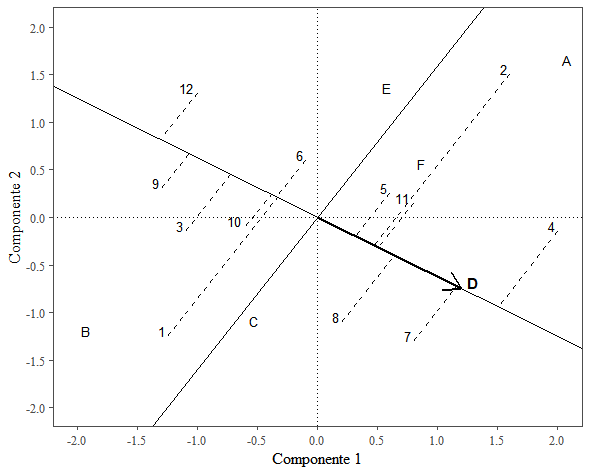
\includegraphics[width=10cm]{./Graficos/env_GGE.png}
	\end{center}
	\caption{Ranking de genotipos en el ambiente D a través del biplot GGE}
	\label{fig:fig312}
\end{figure}


Los marcadores de los genotipos 4, 7, 8, 11, 2 y 5 quedan del lado del marcador del ambiente D, de acuerdo a la división de la perpendicular que pasa por el origen, por que se interpreta que estos genotipos tienen un rendimiento mayor al promedio del ambiente D. Los restantes genotipos tienen un rendimiento inferior al promedio.


Para visualizar el desempeño de un genotipo en los diferentes ambientes, Yan y Hunt (2002) sugieren graficar una línea que una el marcador del genotipo con el origen y luego trazar otra línea perpendicular a la primera. Esta última perpendicular es la que separa los sitos favorables y desfavorables para el genotipo. Los sitios cuyos marcadores queden en el mismo lado donde está el genotipo son los mejores para ese genotipo y los restantes son aquellos donde el genotipo rinde por debajo de su promedio.



Como se puede apreciar en la Figura \ref{fig:fig313}, la perpendicular al marcador del genotipo 2, determina que los ambientes favorables para ese genotipo son A, E, F y D, en donde el mismo tiene rendimientos mayores a su promedio. Los ambientes desfavorables son B y C.
También se observa que el ambiente más favorable es el A, luego le siguen el E y el F. Si bien el ambiente D también es favorable, en ese ambiente el rendimiento del genotipo 2 es apenas superior a su rendimiento medio ya que el marcador del ambiente D, está muy cerca de la perpendicular que pasa por el origen.

\begin{figure}[h]
	\begin{center}
		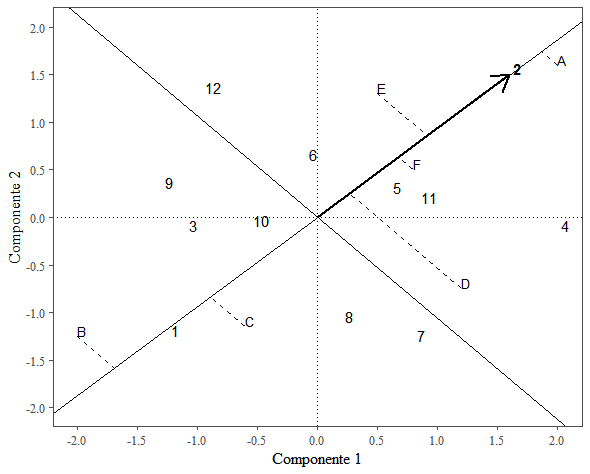
\includegraphics[width=10cm]{./Graficos/gen_GGE.png}
	\end{center}
	\caption{Ambientes favorables y desfavorables para el genotipo 2 en el biplot GGE}
	\label{fig:fig313}
\end{figure}


Para comparar dos genotipos, se propone unir mediante una línea recta los genotipos a comparar, luego trazar una línea que pase por el origen y que sea perpendicular a la línea que une a los genotipos. Esta última línea es la que separa sitios favorables a uno y a otro genotipo.


Los sitios cuyos marcadores queden en el mismo lado donde está el marcador del genotipo son los mejores para ese genotipo. Si un ambiente queda posicionado sobre la línea perpendicular, los dos genotipos tienen rendimientos similares en ese ambiente. Si dos genotipos están cercanos, sus rendimientos son similares en los ambientes evaluados. Por último, si todos los ambientes quedan a un lado de la línea perpendicular, el genotipo cuyo identificador está de ese lado rinde más que el otro en todos los ambientes.
En la Figura  \ref{fig:fig314} se puede ver la comparación de los desempeños de los genotipos 6 y 8. Los ambientes que resultan favorables para el genotipo 6 son el E, el A y el F. Mientras que los favorables para el genotipo 8 son el B, el C y el D.

\begin{figure}[h]
	\begin{center}
		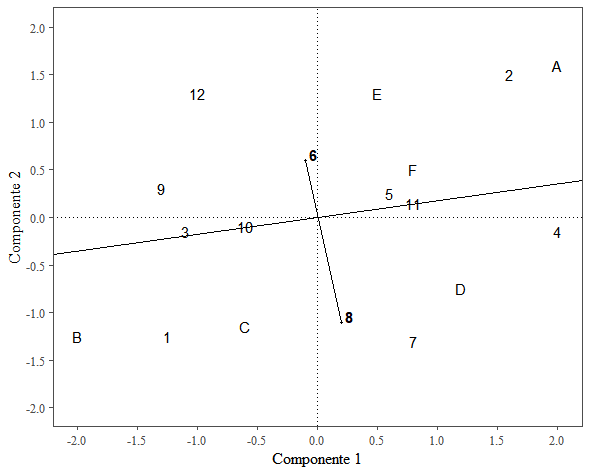
\includegraphics[width=10cm]{./Graficos/comp_gen_GGE.png}
	\end{center}
	\caption{Comparación de los genotipos 6 y 8 en el biplot GGE}
	\label{fig:fig314}
\end{figure}


Para poder identificar mega-ambientes y los mejores genotipos en cada uno de ellos se propone graficar un polígono envolvente. Este polígono se forma uniendo los genotipos más extremos en el biplot con segmentos continuados. Luego se trazan líneas rectas que pasan por el origen y que son perpendiculares a cada uno de los lados del polígono (o a sus proyecciones). De esta forma, el biplot queda dividido en cuadrantes, y los sitios que quedan dentro un mismo cuadrante se consideran pertenecientes a un mismo mega-ambiente. Generalmente cada cuadrante contiene un genotipo en el vértice, que es el de mayor rendimiento en el mega-ambiente.
En la Figura \ref{fig:fig315} se presenta el biplot GGE con el polígono envolvente y las perpendiculares a sus lados, que ayudan a la interpretación del mismo.

\begin{figure}[h]
	\begin{center}
		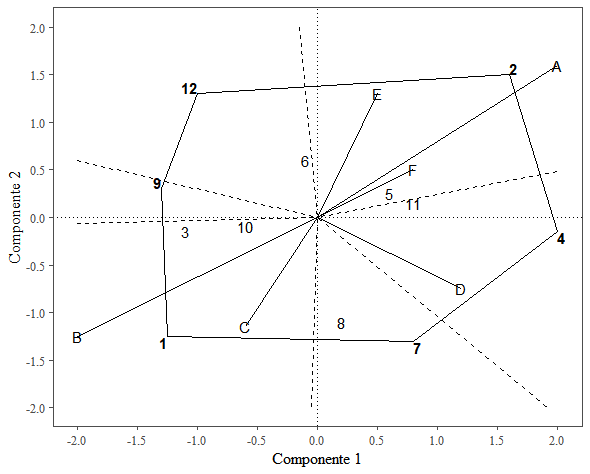
\includegraphics[width=10cm]{./Graficos/poligono_GGE.png}
	\end{center}
	\caption{Biplot GGE con el polígono envolvente y las perpendiculares a sus lados}
	\label{fig:fig315}
\end{figure}


En primer lugar se observa que los marcadores de los ambientes A y B son mayores a los restantes, lo que indica que la variabilidad en esos ambientes es superior, es decir, en ellos es donde mejor se diferencian los efectos de los genotipos.
Las perpendiculares a los lados del polígono envolvente determinan tres mega-ambientes:
\begin{itemize}
\item uno formado por los ambientes A, E y F, en donde el genotipo de mejor desempeño es el 2 (se
encuentra en el vértice del polígono encerrado por las perpendiculares).
\item otro está formado solo por el ambiente D y el genotipo ganador en él es el 4, y
\item  el tercer mega-ambiente lo componen los ambientes B y C, en este caso el genotipo ganador es el 1.
\end{itemize}

Si se identifican distintos mega-ambientes, la selección de genotipos debe hacerse para cada mega-ambiente en particular. Los genotipos se seleccionan en base a su desempeño y a su estabilidad a través de los ambientes.
En el biplot, se puede definir un eje medio para todos los ambientes pertenecientes a un mismo mega-ambiente. Para ello se calcula la media de scores promediando los scores de la componente 1 y la componente 2 de los ambientes pertenecientes al mega-ambiente. Una vez obtenidos estos promedios, se traza una línea recta entre ese punto medio y el origen, que se denomina eje de la media de scores de ambientes. A continuación se traza una línea que pase por el origen y que sea perpendicular a la línea
media de scores de ambientes. Estas dos líneas constituyen ``el eje de coordenadas de ambiente medio''.
Las proyecciones de los marcadores de los genotipos sobre el eje de la media de scores de ambientes da un ranking de los rendimientos de los genotipos en ese mega-ambiente. A su vez la magnitud de la proyección de los marcadores de los genotipos a la perpendicular al eje de ambientes da una idea de la estabilidad. Cuanto mayor sea esta magnitud, más inestable será el genotipo.
En este ejemplo se calcula el ambiente medio para un mega-ambiente, en la Figura 4.6 se presenta el gráfico del eje medio para el mega-ambiente formado por los ambientes A, E y F. El promedio de los scores de la primer componentes es 1,00 y el de la segunda es 1,133, por lo que el punto medio que determina la dirección del eje es (1; 1,133), que está graficado con un círculo en la Figura \ref{fig:fig316}.

\begin{figure}[h]
	\begin{center}
		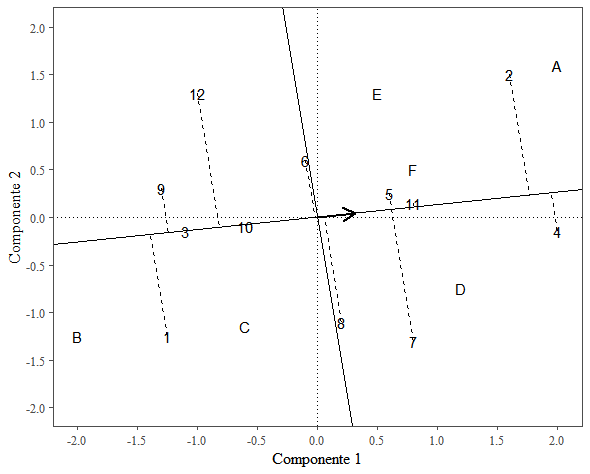
\includegraphics[width=10cm]{./Graficos/mean_stab_GGE.png}
	\end{center}
	\caption{Eje de coordenadas de ambiente medio para un mega-ambiente en el biplot GGE}
	\label{fig:fig316}
\end{figure}

Como se puede observar en el biplot el orden de los genotipos (de mayor a menor rendimiento) es: 2, 4, 12, 11, 5, 6 todos ellos con rendimientos superiores al promedio, seguidos por los de rendimiento menor al promedio: el 10, 9, 7, 3 y por último el 1, el de peor rendimiento medio en ese mega-ambiente.
Debido a que las proyecciones sobre el eje perpendicular al eje medio de ambiente dan una idea de la estabilidad, se observa que el genotipo 12, el 9, el 7 y el 4 son los más inestables. También se observa que el genotipo 2, además de tener el mejor rendimiento medio es de los más estables en el megaambiente.


\subsection{Métodos de imputación}




\section{Paquete de R}

%https://oscarperpinan.github.io/R/Paquetes.html 
Una librería o paquete (\emph{package}) es una colección de objetos creados y organizados siguiendo un protocolo fijo que garantiza un soporte mínimo para el usuario así como la ausencia de errores (de sintaxis) en la programación.

\subsection{Creación del paquete de R}
Los pasos necesarios para la creación de un paquete son:
\begin{itemize}
\item Creación de los objetos que contendrá el paquete (funciones y/o
datos).
\item Creación del esqueleto del paquete.
\item Redacción de la documentación.
\item Compilación del paquete en Linux y creación de la versión para Windows.
\item Instalación.
\item Prueba y publicación.
\end{itemize}

\subsubsection{Objetos del paquete}
Un paquete puede contener cualquier tipo de objetos de R : funciones, datos etc. Lo primero que debe hacerse es programar las funciones y preparar los datos. El proceso de creación vigila que no hayan errores sintácticos pero no controla si hay errores lógicos.
 
\subsubsection{Esqueleto y estructura del paquete}
R proporciona una función \emph{package.skeleton} que permite automatizar el proceso de creación de un paquete creando los directorios, los archivos de documentación y otros objetos necesarios.
La  siguiente instrucción construye la estructura de un paquete llamado \emph{geneticae}, 

\begin{lstlisting}[frame=single]
package.skeleton(name = geneticae)
\end{lstlisting}

creando una carpeta de nombre \emph{geneticae} con 3 sub-carpetas en el directorio de trabajo y tres archivos sin extensión. Estos ultimos son los siguintes: 
\begin{itemize}

\item DESCRIPTION: contenido básico para
documentar según la descripción del paquete:

Package: geneticae\\
Type: Package\\
Title: What the package does (short line)\\
Version: 1.0\\
Date: 2019-09-21\\
Author: Who wrote it\\
Maintainer: Who to complain to <yourfault@somewhere.net>\\
Description: More about what it does (maybe more than one line)\\
License: What license is it under?\\

\item NAMESPACE: R usa un sistema de gestión de espacio de nombres que permite al autor del paquete especificar:
\begin{itemize}
\item las variables del paquete que se exportan (y son, por tanto, accesibles a los usuarios)
\item las variables que se importan de otros paquetes.
\item las clases y métodos S3 y S4 que deben registrarse.
\end{itemize}

Este mecanismo queda definido en el contenido del fichero NAMESPACE.

\item Read-and-delete-me: contiene algunas instrucciones importantes sobre cómo personalizar el paquete.
\end{itemize}

Las siguientes son las 3 sub-carpetas creadas:

\begin{itemize}
\item La carpeta \textbf{data} contiene todos los archivos correspondientes a los datos comprimidos con el nombre con el que fueron creados, con la extensión .rda. Estos no pueden ser modificados.
\item La carpeta \textbf{man} contiene todos los archivos de extensión .Rd y un archivo por objeto creado (datos o programa). Estos documentos son parte del sistema de ayuda del paquete en PDF y en HTML; por este motivo, la escritura sigue las reglas de LaTeX.
\item La carpeta \textbf{R} contiene todos los programas fuente, siendo .R la extensión de los mismos.
\end{itemize}
La documentación es uno de los aspectos mas importantes del código, sin ella, los usuarios no sabrán cómo usar el paquete. R proporciona una forma estándar de documentar paquetes: escribir archivos .Rd en la carpeta man, los cuales utilizan una sintaxis personalizada, basada en LaTeX. Sin embargo, el paquete \emph{roxygen2}, utilizado en este trabajo, permite obtener la documentación de una manera sencilla, proporcionando una serie de ventajas sobre la escritura los archivos .Rd:

\begin{itemize}
\item El código y la documentación son adyacentes, de modo que cuando el código se modifique, será fácil actualizar la documentación.

\item Inspecciona dinámicamente los objetos que está documentando, para que pueda agregar automáticamente los datos que de otra forma se deben escribir a mano.

\item Resume las diferencias en la documentación de los métodos S3 y S4, los genéricos y las clases, por lo que necesita aprender menos detalles.
\end{itemize}

Además de generar archivos .Rd, \emph{roxygen2} también creará un archivo NAMESPACE y administrará el campo \emph{Imports} del archivo DESCRIPTION.


\subsubsection{Compilación e instalación}
Una vez creada la documentación se debe chequear el paquete y generar los instaladores con su corresponiente manual. Para ello se utilizan las siguiente funciones:
\begin{itemize}
\item \emph{R CMD check} verificará que no haya errores de sintaxis o no se generen warnings. Está compuesto por más de 50 chequeos individuales entre los cuales se encuentran: la estructura del paquete, el archivo descripción, namespace, el código de R, los datos, la documentación, entre otros.
\item  \emph{R CMD build} compilará el paquete generando un archivo geneticae.tar.gz listo para su instalación en Linux y \emph{RCMD build -binary} generará el archivo para la instalación en Windows.
\item \emph{RCMD Rd2dvi --pdf} preparará el manual y \emph{R CMD INSTALL} instalará el paquete dejándolo listo para su uso
\end{itemize}

\subsubsection{Publicación}
%https://rsanchezs.gitbooks.io/ciencia-de-datos-con-r/paquetes/paquetes.html
Un repositorio es el lugar dónde están alojados los paquetes y desde el cuál se pueden descargarlos. Entre los repositorios más populares de paquetes R se encuentran:

\begin{itemize}
\item \textbf{CRAN}: es el principal repositorio de paquetes de R, está coordinado por la fundación R. Previa a la publicación en este repositorio el paquete debe pasar por diferentes pruebas para asegurar que cumple con las políticas de CRAN.

\item \textbf{Bioconductor}: se trata de un repositorio específico para bioinformática. Del mismo modo que CRAN, tiene sus propias políticas de publicaciones y procesos de revisión.

\item \textbf{GitHub}: a pesar que no es específico para R, github es con toda seguridad el repositorio más popular para la publicación de proyectos \emph{open source} (del inglés, código abierto). Su popularidad procede del espacio ilimitado que proporciona para el alojamiento de proyectos \emph{open source}, la integración con git (un software de control de versiones) y, la facilidad de compartir y colaborar con otras personas. Una de sus desventajas es que no proporciona procesos de control.

\item \textbf{R-Forge} y \textbf{RForge}: son entornos de desarrollo de paquetes y repositorios. Eso significa que incluyen control de fuente, seguimiento de errores y otras características. Puede obtener versiones de desarrollo de paquetes de estos.
\end{itemize}

El paquete \emph{geneticae} se encuentra en GitHub, para instalar el mismo (o cualquiera que se encuentre en dicho repositorio) se deben seguir las siguientes instrucciones:\\


\begin{lstlisting}[frame=single]
install.packages(remotes) 
library(remotes)
install_github(jangelini/geneticae) 
\end{lstlisting}


{\Huge{FALTAN LAS COMILLITAS EN INSTALL Y EN EL USUARIO DE GITHUB.. ME DA ERROR CUANDO LAS PONGO}}



{\Huge{(Ideas de: TRABAJO FINAL P SHINY)}}

\section{Shiny APP}
Una aplicación web es una aplicación o herramienta informática accesible desde cualquier navegador, bien sea a través de internet (lo habitual) o bien a través de una red local. 
Estas aplicaciones son muy populares hoy en día para los usuarios no expertos, debido a la facilidad de su uso, ya que no es preciso instalar nada en el ordenador, simplemente se accede a través de un navegador. Además se puede acceder desde cualquier dispositivo con conexión a internet, ya sea un ordenador, un smartphone o una tablet, es decir que es independiente del sistema operativo del usuario. Otra gran ventaja es el bajo consumo de recursos, ya que la mayor parte del tiempo estos se consumen en el servidor donde se encuentra alojada la aplicación, que generalmente tiene mucha más potencia de cómputo que cualquier ordenador personal.

%https://datanalytics.com/libro_r/shiny.html
Shiny es un paquete, que se encuentra instalado por defecto con Rstudio, con el que se pueden desarrollar aplicaciones web interactivas, directamente desde Rstudio sin necesitar conocimientos de HTML, CSS o Javascript. Shiny implementa la programación reactiva (cita de archivo aplicacion shiny) en donde los objetos (gráficos y tablas) que forman la aplicación responden a los inputs de los usuarios, dotando a estos de una gran capacidad de control.

En general, en estas aplicaciones, se distinguen tres pasos en el funcionamiento de la aplicación:
\begin{enumerate}
\item El usuario modifica todos aquellos widgets que quedan a su disposición en el navegador (los llamaremos inputs).
\item Los valores de los inputs se envían a R que realiza los análisis indicados.
\item Los resultados de estos cálculos se muestran en el navegador (los llamaremos outputs).
\end{enumerate}

El esquema interno de la aplicación puede observarse en la Figura \ref{fig:fig321}. 

\begin{figure}[h]
\begin{center}
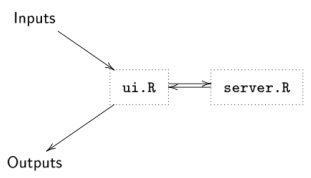
\includegraphics[width=7cm]{./Graficos/figura7}
\end{center}
\caption{Esquema interno de la aplicación.}
\label{fig:fig321}
\end{figure}


En las páginas y aplicaciones web se ha estandarizado el uso de ciertos lenguajes, tales como HTML, CSS, PHP o Javascript entre otros. Por defecto Shiny utiliza una plantilla básica de Twitter Bootstrap [18] para crear la interfaz de usuario, pero podemos descargar otras plantillas o crear una propia para personalizar nuestra aplicación. Twitter Bootstrap es un entorno de trabajo desarrollado por empleados de Twitter para fomentar la consistencia entre las herramientas internas, de forma que todas siguieran el mismo estilo. En 2011 Twitter liberó Bootstrap como código abierto, permitiendo que cualquiera lo usara para diseñar sus sitios o aplicaciones web. Contiene elementos de diseño basado en HTML, CSS y Javascript. Una de las mayores ventajas de Bootstrap es que permite crear interfaces web con CSS y JavaScript que adaptan la interfaz dependiendo del tamaño del dispositivo en el que se visualice de forma nativa, es decir, automáticamente se adapta al tamaño de un ordenador o de una tablet sin que el usuario tenga que hacer nada. Esto se denomina diseño adaptable o Responsive Design.

En lugar de usar un CSS propio para la interfaz de la aplicación se ha usado el paquete de R shinythemes [8], publicado por los creadores del propio Shiny. Shinytemes ofrece una serie de estilos básicos para aplicaciones Shiny.



\subsection{Creación de la Shiny APP}
%http://www.rpubs.com/JohanMarin/Shiny
La instalación de este paquete puede realizarse a través de los menús de Rstudio o simplemente con la siguiente orden:\\

\begin{lstlisting}[frame=single]
install.packages(shiny)
\end{lstlisting}

Para crear una Shiny app en \emph{File} se elige la opción Shiny Web App (figura \ref{fig:fig322}).

\begin{figure}[h]
\begin{center}
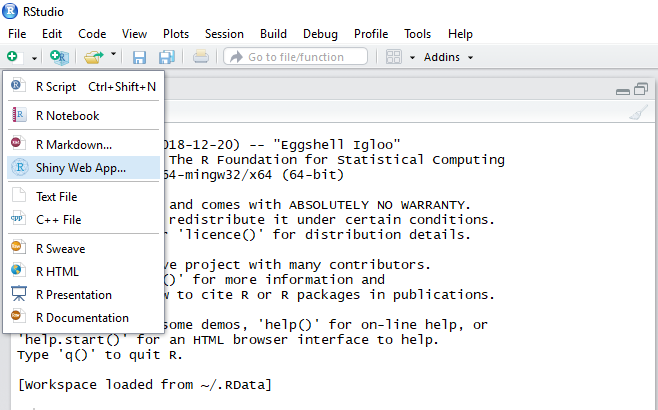
\includegraphics[width=12cm]{./Graficos/figura4}
\end{center}
\caption{Creación de Shiny Web App desde Rstudio}
\label{fig:fig322}
\end{figure}


Las aplicaciones Shiny están compuestas por un archivo app.R o dos archivos ui.R y server.R, es decir, se puede partir de un solo fichero que aglutine todo el código o se puede partir de dos archivos que separan la parte cliente de la parte servidora.

En este trabajo, se crea la aplicación Shiny mediante un unico script llamado app.R. El mismo se encuentra en un directorio (por ejemplo newdir/) y la aplicación se puede ejecutar con runApp(``newdir''). El script app.R esta formado por tres componentes:

\begin{itemize}
\item ui (\emph{user interfaz}): la interfaz de usuario controla el diseño de la aplicación, recibe los inputs y
muestra los outputs en el navegador.
\item server, funciones de R que contienen las instrucciones que se necesitan para construir los resultados de los análisis incluidos en la aplicación.
\item shinyApp, función que crea objetos de aplicación Shiny a partir de ui / servidor.
\end{itemize}


El archivo app.R deberá comenzar cargando el paquete Shiny y finalizar con una llamada a shinyApp:\\

\begin{lstlisting}[frame=single]
library(shiny)
ui<- ...
server<- ...
shinyApp(ui = ui, server = server)
\end{lstlisting}

La sesión de R estará monitoreando la aplicación y ejecutando las reacciones de la aplicación mientras la aplicación Shiny esté activa, por lo que no podrá ejecutar ningún comando.

La Figura \ref{fig:fig323} muestra el diseño utilizado en la aplicación. Se cuenta con un titulo y diferentes pestañas que conducen a diferentes páginas de la aplicación (\textbf{A}). Se cuenta con un panel de barra lateral (\textbf{B}), que contiene principalmente widgets con los cuales el usuario puede determinar el análisis que desea realizar y un panel principal (\textbf{C}) en el cual se obtenene los resultados del análisis solicitado.

\begin{figure}[h]
\begin{center}
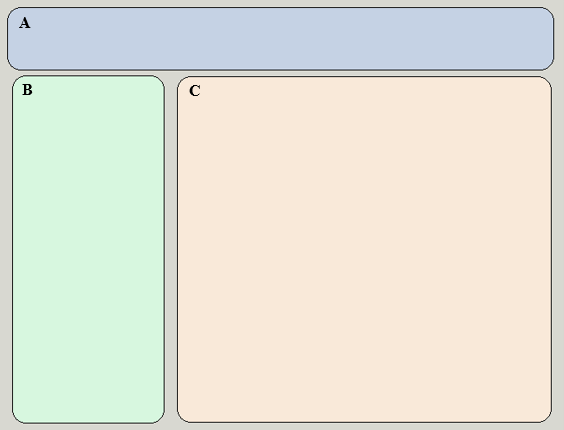
\includegraphics[width=12cm]{./Graficos/figura6}
\end{center}
\caption{Diseño de la aplicación Shiny. \textbf{A}: título y pestañas; \textbf{B}: área de entrada; \textbf{C}: área de resultados.}
\label{fig:fig323}
\end{figure}

\subsubsection{Tipos de componentes de Shiny Web App}

Los tipos de componentes de una aplación Shiny son:
\begin{itemize}
\item Componentes de Inputs y Outputs. Entre los inputs se encuentran numericInput, sliderInput, textInput, checkboxInput, entre otros. Posibles outputs se encuentran en la tabla \ref{tab:tabla1}, con las correspondientes funciones para server.R y ui.R
\item Componentes de Diseño. Algunos ejemplos se muestra en la tabla \ref{tab:tabla2}.
\item Componentes HTML (tags).
\end{itemize}


\begin{table}[h]
\begin{center}
\caption{Funciones para Outputs tanto para server.R como para ui.R}
\label{tab:tabla1}
\resizebox{\textwidth}{!} {
\begin{tabular}{cccc}
\hline
server.R & ui.R & espera & crea \\
\hline 
renderPlot & plotOutput & Gráfica & Gráfica\\
renderPrint & verbatimTextOutput, htmlOutput& salida impresa & texto\\
renderTable & tableOutput & objetos como tablas & tabla simple\\
renderDataTable & dataTableOutput & objetos como tablas & tabla DataTables.js\\
downloadHandler	& downloadButton, downloadLink & &\\
\hline 
\end{tabular}
}
\end{center}
\end{table}

\subsubsection{Componentes de Diseño}
% http://rstudio-pubs-static.s3.amazonaws.com/21373_8af3d3634b97461089c8a76659982915.html#componentes-shiny
\begin{itemize}
\item navbarPage(): Crea una página con una barra de navegación de nivel superior.
\item tabPanel(): Crea un panel de pestañas.
\item sidebarLayout(): Diseña de una barra lateral y el área principal.
\item sidebarPanel(): Crea un panel de barra lateral.
\item mainPanel(): Crea un panel principal.
\item navlistPanel(): Crea un panel de lista de navegación.
\item prettyRadioButtons(): Crea botones que permiten seleccionar un elemento de una lista.
\item materialSwitch(): Crea un interruptor de palanca para activar o desactivar una selección.
\item pickerInput(): Crea un control de selección de entrada.
\item navbarMenu():
\end{itemize}

{\small
\begin{table}[h]
\begin{center}
\caption{Componentes de Diseño de Shiny Web App}
\label{tab:tabla2}
\resizebox{0.6\textwidth}{!} {
\begin{tabular}{cccc}
\hline 
Componente	& Subcomponente	 \\
\hline
navbarPage(): & tabPanel(), navbarMenu()\\
navbarMenu() & tabPanel() \\
navlistPanel() & tabPanel()\\
titlePanel() &	\\
sidebarLayout() & sidebarPanel()  mainPanel() (obligatorio)	\\
sidebarPanel() & \\
mainPanel() & \\
tabsetPanel() &	\\
tabPanel()	 & \\
\hline
\end{tabular}
}
\end{center}
\end{table}
}


Para más información sobre estas componentes ver hoja de referencia de Shiny (Apéndice A).


\subsubsection{Compartiendo una Shiny Web App}

Una vez creada la aplicación, resulta conveniente ponerlas a disposición de los usuarios. En este caso la Shiny Web App encuentra disponible en el servidor de CONICET \url{www.cefobi.com}. Además el proyecto se encuentra en GitHub \url{https://github.com/jangelini/shinyAPP_geneticae}. 
